\documentclass[a4paper,11pt]{article}

%---enable russian----

\usepackage[utf8]{inputenc}
\usepackage[russian]{babel}
%\usepackage[T2A]{fontenc}


\usepackage{graphicx}
\usepackage{url}
\usepackage{latexsym}
\usepackage{amscd,amsmath,amsthm,euscript}
\usepackage{mathtools}
\usepackage{amsfonts}
\usepackage{amssymb}
\usepackage[dvipsnames]{xcolor}
\usepackage{hyperref}
\usepackage{algorithm}
\usepackage[noend]{algpseudocode} 




\newtheorem{theorem}{Теорема}
\newtheorem{corollary}[theorem]{Следствие}
\newtheorem{lemma}[theorem]{Лемма}
\newtheorem{observation}[theorem]{Замечание}
\newtheorem{proposition}[theorem]{Предложение}
\newtheorem{definition}[theorem]{Определение}
\newtheorem{claim}[theorem]{Утверждение}
\newtheorem{fact}[theorem]{Факт}
\newtheorem{assumption}[theorem]{Предположение}

% 1-inch margins
\topmargin 0pt
\advance \topmargin by -\headheight
\advance \topmargin by -\headsep
\textheight 8.9in
\oddsidemargin 0pt
\evensidemargin \oddsidemargin
\marginparwidth 0.5in
\textwidth 6.5in

\parindent 0in
\parskip 1.5ex

%%All notations/commands
% ==================================================================
% Definitions for this paper
% ==================================================================
\mathchardef\hyphen="2D

\usepackage{multirow}
\usepackage{multicol} % For multiple coloumn environments
%\usepackage{stmaryrd} % For set brackets
% \setlength{\columnsep}{15pt} % Defining the coloumn seperation
% \setlength{\columnseprule}{1pt} % Place a line between coloumns
% \newcommand{\tab}{\hspace*{2em}}

% ADVERSARIES AND SUCH
% \newcommand{\advA}{\mathcal{A}} % Adversary 
% \newcommand{\advB}{\mathcal{B}} % Simulator
% \newcommand{\advC}{\mathcal{C}} % Challenger
% \newcommand{\advD}{\mathcal{D}} % Distinguisher
% \newcommand{\advF}{\mathcal{F}} % Forger
% \newcommand{\advI}{\mathcal{I}} % Invertor
% \newcommand{\advR}{\mathcal{R}} % Reduction


% GROUPS/DISTRIBUTIONS/SETS/LISTS
% \newcommand{\msgspace}{\mathfrak{M}} % Message space
% \newcommand{\keyspace}{\mathfrak{K}} % Key Space
% \newcommand{\sigspace}{\mathfrak{S}} % Signature Space
% \newcommand{\ctspace}{\mathfrak{C}} % Ciphertext Space
% \newcommand{\prm}{\mathbb{P}} % Set of prime numbers
\newcommand{\N}{{{\mathbb N}}}
\newcommand{\Z}{{{\mathbb Z}}}
\newcommand*{\Q}{\mathbb{Q}}
\newcommand{\R}{{{\mathbb R}}}
\newcommand{\F}{{{\mathbb F}}}
%\newcommand{\T}{\mathbb{T}} % Additive group of reals mod 1: R/Z
% \newcommand{\dis}{\mathfrak{D}} % Distributions
% \newcommand{\grp}{\mathbb{G}} % Group
% \newcommand{\inr}{\in_{_R}} % Uniformily random in
% \newcommand{\rnd}{\leftarrow_{\mbox{\tiny{\$}}}} % Randomised algorithm output
\newcommand{\getsr}{\mathbin{\leftarrow_{\mbox{\tiny{\$}}}}} % Randomised algorithm output
% \newcommand{\intval}[1]{\llbracket #1 \rrbracket} % Int val
% \newcommand{\qlist}{\mathcal{Q}}
\newcommand{\LWEErrorDist}{\ensuremath{D}}
\newcommand{\transpose}{\mkern0.7mu^{\mathsf{ t}}}
\newcommand{\Ball}{\mathcal{B}} % Ball
\newcommand{\Image}{\text{Im}} % Image of an operator
\newcommand*{\poly}{\ensuremath{\mathrm{poly}}}
\newcommand*{\eps}{\ensuremath{\varepsilon}}
\renewcommand{\d}{\mathrm{d}}
\DeclareMathOperator*{\E}{\mathbb{E}} %Expectation
\newcommand*{\union}{\mathbin{\cup}} %union

%ordinal numbers
\renewcommand{\th}{^{\mathrm{th}}}
%\newcommand{\st}{^{\mathrm{st}}}
\newcommand{\nd}{^{\mathrm{nd}}}

%{0,1}^n
\newcommand*{\ZO}[1]{\ensuremath{\{0,1 \}^{#1}}}



%Fancy Roman numerals
\def\barroman#1{\sbox0{#1}\dimen0=\dimexpr\wd0+1pt\relax
  \makebox[\dimen0]{\rlap{\vrule width\dimen0 height 0.06ex depth 0.06ex}%
    \rlap{\vrule width\dimen0 height\dimexpr\ht0+0.03ex\relax 
            depth\dimexpr-\ht0+0.09ex\relax}%
    \kern.5pt#1\kern.5pt}}


%%% LWE
\newcommand{\LWEDist}{\mathcal{A}_{\vec s, \chi}}
%\newcommand{\cq}{\ensuremath{c_\protect\SmallTextScript{1}{{q}}}}

%Constants
\newcommand{\cq}{\ensuremath{\mathsf{c}_q}}
\newcommand{\ca}{\ensuremath{\mathsf{c}_{\alpha}}}
\newcommand{\cm}{\ensuremath{\mathsf{c}_m}}
\newcommand*\cBKZ{c_{\mkern-1.5mu\protect\SmallTextScript{0.8}{\BKZ}}}
\newcommand{\cf}{\ensuremath{\mathsf{c}_f}}
\newcommand{\cg}{\ensuremath{\mathsf{c}_{\gamma}}}
%\newcommand{\const}{\mathsf{c}} 

\newcommand{\B}{\mathfrak{B}} %family of bounding functions
\newcommand*\Dmax{D_{\max}} %max distance 

\newcommand*\Enq[2]{{#1}.\mathsf{Enqueue}({#2})}
\newcommand*\Deq[1]{{#1}.\mathsf{Dequeue}()}
\newcommand{\counter}{\mathsf{cntr}}
\newcommand*\nNodes{\mathrm{\#N}} %Number of nodes
\newcommand*\nT{\mathrm{\#NThreads}} %Number of threads
\newcommand*{\im}{\ensuremath{i_{\mkern-1.5mu\protect\SmallTextScript{0.7}{\textup{max}}} \mskip -1.5mu }} %i_max

%%% ALGORITHMS/PROCEDURES/PROBLEMS %%%
\newcommand{\BDD}{\textsf{BDD}\xspace}
\newcommand{\ALG}{\texttt{ALG}\xspace}
\newcommand{\DUAL}{\texttt{Dual}\xspace}
\newcommand{\ENUM}{\texttt{Enum}\xspace}
\newcommand{\SVP}{\textsf{SVP}\xspace}
\newcommand{\appSVP}{\ensuremath{\textsf{appSVP}_{\gamma}}\xspace}
\newcommand{\uSVP}{\ensuremath{\textsf{uSVP}_{\gamma}}\xspace}
\newcommand{\CVP}{\textsf{CVP}\xspace}
\newcommand{\BKZ}{\texttt{BKZ}\xspace}
\newcommand{\LLL}{\texttt{LLL}\xspace}
\newcommand{\BKW}{\texttt{BKW}\xspace}
\newcommand{\BKWKF}{\texttt{BKW2}\xspace}
\newcommand{\LWE}{\textsf{LWE}\xspace}
\newcommand{\SIS}{\textsf{SIS}\xspace}
\newcommand{\SIVP}{\textsf{SIVP}\xspace}
\newcommand{\HKZ}{\textsf{HKZ}\xspace}
\newcommand{\LPN}{\textsf{LPN}\xspace}
\newcommand*\GenPrun{\texttt{GenPruning}\xspace}
\newcommand*\GenPrunDepth{\texttt{GenPruningDepthFirst}\xspace}
\newcommand*\GP{\texttt{GP}\xspace}
\newcommand*\NP{\texttt{NearestPlane}\xspace}
\newcommand*\NPs{\texttt{NearestPlane\underline{s}}\xspace}
\newcommand{\fplll}{\texttt{fplll}\xspace}
\newcommand{\AKS}{\textsf{AKS}\xspace}

\newcommand*\Embed{\texttt{Embed}\xspace}
\newcommand*\Dual{\texttt{Dual}\xspace}
\newcommand*\DualC{\texttt{Dual}^{1}\xspace}

\newcommand*\SubBabai{{\mbox{\tiny Babai}}}
\newcommand*\SubLP{{\mbox{\tiny LP}}}
\newcommand*\SubGenPruning{{\mbox{\tiny GP}}}

\newcommand*{\ENUMOne}{\ENUM_{\protect\SmallTextScript{0.8}{1}}}
\newcommand*{\ENUMH}{\ENUM_{\protect\SmallTextScript{0.7}{0.292}}}

\newcommand*{\DUALOne}{\DUAL_{\protect\SmallTextScript{0.8}{1}}}
\newcommand*{\DUALH}{\DUAL_{\protect\SmallTextScript{0.7}{0.292}}}

%Landau and such

\newcommand{\bigO}{\mathcal{O}}
\newcommand{\smallo}{o} 
\newcommand{\wLandau}{\omega}
\newcommand{\negl}{\mathrm{negl}}
\newcommand*{\WLandau}{\varOmega}
\newcommand*{\softO}{\widetilde{\bigO}}
\newcommand*{\softOmega}{\widetilde{\WLandau}}
\newcommand*{\TLandau}{\varTheta}
\newcommand*{\xTLandau}{\widetilde{\TLandau}}
\newcommand*\PROB\Pr 
\newcommand*\Psucc{P\mkern-4mu_{\mbox{\tiny succ}}}
\DeclareMathOperator*{\EXPECT}{\mathbb{E}}
\DeclareMathOperator*{\VARIANCE}{\mathbb{V}}
\DeclareMathOperator*{\LOGBIAS}{\mathbb{LB}}
\DeclareMathOperator*{\low}{\mathrm{low}}


%Matrices and Vectors
\newcommand{\AMat}{\ensuremath{A}}
\newcommand{\BMat}{\ensuremath{B}}
\newcommand{\wBMat}{\ensuremath{B^*}}
\newcommand{\DMat}{\ensuremath{D}}
\newcommand{\UMat}{\ensuremath{U}}
\newcommand{\XMat}{\ensuremath{X}}
\newcommand{\Id}{\ensuremath{\mathbbm{1}}}
\newcommand{\ZeroM}{\ensuremath{\mathbbm{0}}}

%\renewcommand{\vec}[1]{\vec{#1}\mkern2mu\vphantom{#1}}
\makeatletter
\newcommand{\tvec}{\vec t\@ifnextchar{^}{\,}{\,}}
\newcommand{\svec}{\vec{s}\@ifnextchar{'}{\,}{\,}}
\newcommand{\evec}{\vec{e}\@ifnextchar{'}{\,}{\,}}
\newcommand{\bvec}{\vec b}
\newcommand{\cvec}{\vec c\@ifnextchar{^}{\,}{}}
\newcommand{\xvec}{\vec x}
\newcommand{\vvec}{\vec v\@ifnextchar{^}{\,}{}}
\newcommand{\yvec}{\vec y\@ifnextchar{\ragle}{\,}{\,}}
\newcommand{\zvec}{\vec z}
\newcommand{\zerovec}{\vec 0\@ifnextchar{)}{\,}{\,}}
\newcommand{\onevec}{\vec 1}
\newcommand{\avec}{\vec a}
\newcommand{\dvec}{\vec d}
\newcommand{\pvec}{\vec p\@ifnextchar{'}{\,}{}}
\newcommand{\uvec}{\vec u}
\newcommand{\wvec}{\vec w}

\newcommand{\wbvec}{\vec b^*}
\makeatother

\makeatletter
\newcommand{\evecp}{\vec{e}\@ifnextchar{'}{\,}{}}
\makeatother

% Lattices
\newcommand{\Lat}{\mathcal{L}} %lattice generated as image (rather than kernel).
\newcommand{\LATTp}{\mathcal{L}^{\perp}}
\newcommand*{\qLat}{\mathcal{L}_q} %q-ary lattice
\newcommand*{\qLATTp}{\mathcal{L}_q^{\perp}}
\newcommand*\FP{\smash{\mathcal{P}\mkern-3mu_{\mbox{\tiny 1/2}}}}
\DeclareMathOperator\GSO{GSO}
\newcommand{\LEmb}{\Lat_{\mbox{\tiny Embed}}} %Embedded lattice


%\newcommand{\l1}{\lambda_1} %fist successive minima
% \newcommand{\coset}{\Lambda} % Lambda Lattice
% \newcommand{\cosetPerp}{\Lambda^{\bot}} % Lambda_Perp Lattice
% \newcommand{\gadget}{\textbf{G}} %Gaget matrix
% \newcommand{\mes}{\textbf{m}} %message vector
% \newcommand{\AMat}{\textbf{A}} %A matrices
% \newcommand{\BMat}{\textbf{B}} %B matrices
% \newcommand{\RMat}{\textbf{R}} %R matrices
% \newcommand{\HMat}{\textbf{H}} %H matrices
% \newcommand{\XMat}{\textbf{X}} %H matrices
% \newcommand{\mbar}{\bar{m}} %mBar dimension
% % \newcommand{\gauss}{\mathcal{D}} % gaussian distribution
% \newcommand{\Id}{\textbf{I}} % Identity matrix
% \newcommand{\ZeroM}{\textbf{0}} % Identity matrix
% \newcommand{\er}{\textbf{e}} % gaussian distr. vectors
% % \newcommand{\cipher}{\textit{c}} % ciphertext
% \newcommand{\Olwe}{\mathcal{O}_{\textsf{LWE}}} %LWE oracle
% \newcommand{\OSample}{\mathcal{O}_{Sample}} %LWE oracle
% \newcommand{\SigmaB}{\boldsymbol{\Sigma}} %semi-deifinite matrix Sigma%
% % \newcommand{\mods}{\text{ mod}}


%k-Lists

%\newcommand*{\LL}{\ensuremath{\ell}} %\LL_2 - norm, maybe use $\|.\|$
\newcommand*{\Sphere}[1]{\ensuremath{\mathsf{S}^{#1}}}
\newcommand*{\Conf}{\ensuremath{\text{Conf}\mkern2mu}}
\newcommand*{\ConfSpace}{\ensuremath{\mathscr{C}}}
\newcommand*{\ConfSpacet}{\ensuremath{\mathscr{C}}_{\leq t}}
\newcommand{\Cmax}{\ensuremath{C_{\text{max}}}}
\newcommand*{\pW}{\ensuremath{\rho_{\SmallTextScript{0.8}{\text{Wishart}}}}} %Wishart distribution
\newcommand*{\pC}{\ensuremath{\rho_{\mathscr{C}}}}
%\newcommand*{\Tr}{\ensuremath{\text{Tr}}} % trace
\newcommand*{\Cbal}{\ensuremath{C_{\SmallTextScript{0.8}{\text{B}}}}} %balanced configuration
\newcommand*{\Cbalt}{\ensuremath{C_{\SmallTextScript{0.8}{\text{B,t}}}}} %balanced configuration with target length
\newcommand*{\CbalOne}{\ensuremath{C_{\SmallTextScript{0.8}{\text{B,1}}}}} %balanced configuration with target length 1
\newcommand*{\Lout}{\ensuremath{L_{\mkern-0.5mu\protect\SmallTextScript{0.85}{\textup{out}}}}}

%AppSVP
\newcommand*{\Ei}{\text{E}}



%subscripts

\newcommand*\SmallTextScript[2]{{\mathchoice{\displaystyle #2}%should never be reached
{\textstyle #2}%dito
{\scalebox{#1}{\ensuremath{\scriptstyle #2}}}%
{\scalebox{#1}{\ensuremath{\scriptscriptstyle #2}}}%
}}
% \newcommand*\cq{c_{\protect\SmallTextScript{1}{{q}}}}
% \newcommand*\cs{c_{\protect\SmallTextScript{1}{{s}}}}
% \newcommand*\cBKZ{c_{\mkern-1.5mu\protect\SmallTextScript{0.8}{\BKZ}}}
% \newcommand*\TBKZ{T_{\mkern-1.5mu\protect\SmallTextScript{0.8}{\BKZ}}}
% \newcommand*\MBKZ{\M_{\mkern-0.5mu\protect\SmallTextScript{0.8}{\BKZ}}}


% \newcommand{\rs}{\right]} %right square parenthesis
% \newcommand{\ls}{\left[} %left square parenthesis

% \newcommand{\bL}{\|\bvec_1\|} % b1 length that appears way too often
% \newcommand{\dL}{\|\dvec_1\|} % b1 length that appears way too oftend

%Norms and Scalar products

\newcommand*\abs[1]{\left|#1\right|}
\newcommand*\norm[1]{\left\|#1\right\|}
\newcommand*\normalabs[1]{|#1|} 
\newcommand*\normalnorm[1]{\|#1\|}
\newcommand*\bigabs[1]{\bigl|#1\bigr|}
\newcommand*{\ScProd}[2]{\ensuremath{\langle#1\!\mathbin{,}\!#2\rangle}} %Scalar Product
\newcommand*{\bigScProd}[2]{\ensuremath{\bigl\langle#1\mathrel{,}#2\bigr\rangle}} %Scalar Product
\newcommand*{\BigScProd}[2]{\ensuremath{\Bigl\langle#1\mathbin{,}#2\Bigr\rangle}} %Scalar Product


%Some other math operators

\DeclareMathOperator{\Span}{Span} %span of vectors
\DeclareMathOperator{\vol}{\mathrm{vol}} %volume
\DeclareMathOperator{\LW}{LambertW} %Lambert W function
% \DeclareMathOperator{\Proj}{Proj} %Lambert W function
\DeclareMathOperator{\SD}{SD}
\DeclareMathOperator{\gradient}{grad}




%\DeclareMathOperator{\erf}{erf} %error function
\DeclareMathOperator{\erfc}{erfc} %complementary error function
\newcommand{\Er}{\ensuremath{\mathrm{Er}}} %complementary error function


%Thick line for table
\setlength{\doublerulesep}{0pt}
\newcommand{\thickline}{\hline\hline\hline}


%circled text
\newcommand*\circled[1]{\tikz[baseline=(char.base)]{
    \node[shape=circle,draw,inner sep=0.3 pt] (char) {\scriptsize #1};}}


%Fix Algorithmicx package
\def\NoNumber#1{{\def\alglinenumber##1{}\State #1}\addtocounter{ALG@line}{-1}}

%For Figutes in the ApproxSVP part
\newcommand{\mk}{\mkern-6mu}

%Proper limit with the subscript underneath
% \newcommand{\Lim}[1]{\raisebox{0.5ex}{\scalebox{0.8}{$\displaystyle \lim_{#1}\;$}}}

%enumerates one line of equations inside multiline align*
% \newcommand\numberthis{\addtocounter{equation}{1}\tag{\theequation}}

% Reduc
% \newcommand{\collres}{\mathsf{coll}} % Coll Res
% \newcommand{\dl}{\mathsf{dlog}} % discrete Log
% \newcommand{\Succ}{\mathsf{Succ}}
% \newcommand{\Adv}{\mathsf{Adv}}

%Simplexes
% \newcommand{\simplex}[1]{\triangle^{#1}} %standard simplex
% \newcommand{\trsimplex}[1]{\triangle^{#1}_\text{tr}} %truncated simplex
% \newcommand{\lsimplex}[1]{\triangle^{#1}_\text{lin}} %truncated simplex
% \newcommand{\lksimplex}[1]{\triangle^{#1}_\text{lin,k}} %truncated simplex2  % <<< No packages, only new commands

\begin{document}

\section{Алгоритм Coded-BKW with Sieving}

	
	
	\begin{algorithm}[ph]
		\caption{Coded-BKW with Sieving}
		\label{alg:AlgName}
		\textbf{Вход:}  Матрица $A$ размерности $\Z_q^{n \times m}$, \\
		Полученный вектор $\zvec \in \Z_q^m$, \\
		$t$ - количество шагов,\\
		$C_i$ -- линейный $ [n_i, k_i, d_i]-$ код с быстрым декодером,\\
		$1 \leq i < t$ - индексы,\\
		$B \in \Z$ - параметр \\
		
		\begin{algorithmic}[1]
			
			\State{Изменяется распределение секретного вектора (по методу Гаусса).}\algorithmiccomment{E: этот шаг нуждается в пояснении}
			\For{$i$ from 1 to $t$}
				\For{всех столбцов $h \in H_{i-1}$}
					\State $\Delta=CodeMap(h,i)$
					\State $h$ записывается в список $L_{\Delta}$
				\EndFor
				\For{всех списков $L_{\Delta}$}
					\State $S_{\Delta} = Sieve(L_{\Delta}, i, \sqrt{N_i}\cdot B)$
					\State Все $S_{\Delta}$ записываются в качестве столбцов в $H_i$
				\EndFor
			\EndFor
			\State Происходит угадывание $s_n$ при помощи проверки гипотез.\algorithmiccomment{E: этот шаг тоже нуждается в пояснении}
		\end{algorithmic}
		
	\end{algorithm}
	
\textbf{Замечания к алгоритму:}\\
\begin{enumerate}
\item Полученный на вход вектор $z$ имеет вид $(s,e)\begin{pmatrix} A\\ I \end{pmatrix} = z \Rightarrow (s,e)H_0 = z$, где $H_0 = \begin{pmatrix} A\\ I \end{pmatrix}$, $s$ - секретный вектор в $\Z^{n}_q$, $e$ - вектор ошибок.
\item Константа $B$ обозначает средний уровень «мелкости» для позиции.
\item Опишем процедуру $CodeMap$. В соответствии с основной идеей Coded-BKW, фиксируем код $C_i$ длины $n_i$. Вектор $h$, полученный на входе, сначала считается ограниченным только позициями $N_i+1$ до $N_{i-1}$, т.е. вектор длины $n_i$. Этот вектор, обозначенный $h_{[N_{i-1}+1,N_i]}$, затем отображается в ближайшее кодовое слово в $C_i$. Это ближайшее кодовое слово и обозначается $CodeMap(h,i)$.
\item Опишем процедуру $Sieve$. Полученное на входе $L_{\Delta}$ содержит список векторов. Мы рассматриваем их только первые $N_i$ позиций. Эта процедура найдет разности между любыми двумя векторами такими, что норма разности, ограниченная первыми $N_i$ позициями, меньше, чем $\sqrt{N_i}\cdot B$. Все такие разности отправляются в список $S_{\Delta}$, что и есть результат процедуры. Обычно, список $S_{\Delta}$ содержит примерно столько же векторов, сколько и $L_{\Delta}$. Предполагаем, что векторы в $L_{\Delta}$ ограниченные первыми $N_i$ позициями все имеют норму примерно равную $\sqrt{N_i}\cdot B$. Тогда задача решается алгоритмами просеивания в решетках, например, используя LSH.
\item Этот шаг еще можно назвать “Secret-Noise Transformation”, т.е. Преобразование Секрет-Шум. Его суть состоит в следующем: мы хотим, чтобы секретный вектор следовал тому же распределению $\chi$, что и шум. Процедура работает следующим образом. Сначала мы переписываем матрицу $A$ в т.н. систематической форме (Приводим к такому виду Методом Гаусса). Затем берем первые $n$ линейно независимых столбцов и формируем матрицу $A_0$. Затем находим $D = A_0^{-1}$ и записываем $\hat{s} = sD^{-1} - (z_1,...,z_n)$. Следовательно, мы можем вывести эквивалентную задачу описанную матрицей $\hat{A} = (I, \hat{a}^T_{n+1},..., \hat{a}^T_{m})$, где $\hat{A}=DA$. Вычисляем $\hat{\zvec} = \zvec - (z_1,...,z_n)\hat{A} = (0, \hat{z}_{n+1},..., \hat{z}_{m})$. Используя это преобразование, получаем, что каждая запись в секретном векторе теперь распределена по $\chi$.
\item 	На самом деле, я сам не очень понял этот шаг. В самом начале алгоритма производится т.н. “Initial Guessing Step”, т.е. Шаг Первоначальной Догадки. Выбирается несколько записей $s$, и угадываются их значения (в соответствии с распределением $\chi$). Просматриваются все вероятные значения и производятся для них все остальные шаги алгоритма. Исходя из конкретной догадки, уравнения выборки должны быть переписаны соответствующим образом. Для простоты, оставшиеся неизвестные значения по-прежнему обозначены $s$ и его длина после этого шага по-прежнему обозначается $n$. В самом конце алгоритма (после всех шагов) запускается distinguisher (алгоритм, способный отличить одну выборку от другой) на полученных после работы алгоритма выборках $\zvec$. С помощью него проверяется, была ли верна первоначальная догадка или нет. Но это все относится к началу алгоритма и скорее всего никакой связи с последним шагом (угадывание $s_n$) это не имеет. Честно говоря, мне не помешала бы помощь в понимании этого момента. \footnote{E: Пример. Ваш секретный вектор $\svec$ распределен согласно Гауссовому распределению по п.5. Значит, с высокой вероятностью $s_i \in [-BB,BB]$ для некоторого известного значения $B$ ($B = \const \cdot \alpha q$ для некоторой константы $\const$.)  Для всех возможных значений первой координаты секретного вектора $s_0$, получаем задачу LWE  размерности $n-1$ подстановкой: $(a[1\ldots n-1], b' = b - a_0 s_0 $. Эта задача ``легче'' исходной, так как размерность меньше. Повторяем процесс для каждого возможного значения $s_0 \in [-BB,BB]$. При верном значении $s_0$, алгоритм решения задача LWE восстановит остальные координаты секрета.
Если мы выбираем не одну координату $s_0$, а скажем, $t$ координат, скорость работы такого гибридного алгоритма равна $\bigO(BB^t) \cdot T_{\textup{LWE}(n-r)}$, где $T_{\textup{LWE}(n-r)}$ - время работы алгоритма решения задачи LWE размерности $n-r$.
}
\end{enumerate}

\textbf{Пример первого шага алгоритма:}\\
Столбец $h \in H_0$ сначала попадает в процедуру $\Delta=CodeMap(h,1)$. Затем мы помещаем $h$ в список $L_{\Delta}$. После пробега по всем столбцам $h \in H_0$ они оказываются рассортированными в списки $L_{\Delta}$. Обозначим за $K$ общее число этих списков. Затем пробегаем по всем спискам, каждый содержит примерно $m/K$ столбцов. Производим шаг просеивания  $S_{\Delta} = Sieve(L_{\Delta}, \sqrt{N_1}\cdot B)$, для всех $\Delta \in C_i$. Результатом является список векторов, где норма каждого вектора, ограниченная первыми $N_1$ позициями не превышает $\sqrt{N_1}\cdot B$. Все векторы во всех списках $S_{\Delta}$ теперь помещаются в $H_1$ как столбцы. Теперь мы имеем матрицу $H_1$, где норма каждого столбца, ограниченная первыми $n_1$ позициями, не превышает $\sqrt{N_1}\cdot B$. Конец.

\section{Анализ алгоритма}

Сразу хотел бы сказать, что с пониманием анализа у меня большие проблемы, ибо сам я никогда этим не занимался и даже некоторые обозначения у меня вызывают вопросы. Поэтому отчеты по этой части будут состоять из вопросов, как может показаться, по очевидным вещам.

\textbf{1. Хотелось бы на всякий случай уточнить, что понимается под «магнитудой» (magnitude). Это параметр $B$ } \footnote{E: 
Под ``магнитудой', как правило, понимается норма (Евклидова или $\ell_\infty$). По ходу алгоритма наша задача -- производить вектора  Евклидовой нормы меньше $\leq \sqrt{n_i}B$, следовательно, в конце алгоритма получить вектора Евклидовой нормы $ \leq \sqrt{n}B$. Полагая, что координаты этих векторов примерно равны, мы имеем, что каждая координата полученного вектора $\leqq B$. Заметьте, что этот параметр - свободный и выбирается во время анализа. В итоге, он равен $\poly(n)$
} 

\textbf{2. Разберем самое начало пункта VI PARAMETER SELECTION AND ASYMPTOTIC ANALYSIS до подпункта A.}

После каждого шага, позиции, который уже были обработаны, должны оставаться на некоторой заданной магнитуде $B$. Т.е. среднее (абсолютное значение) обработанной позиции должно быть очень близким к $B$. Это обусловлено тем, что мы применяем просеивание на каждом шаге редукции. После $t$ шагов мы получаем векторы средней нормы $\sqrt{n}\cdot B$.\footnote{E: именно так} 

Зададим число выборок равным ${m=2^k}$, где $2^k$ это параметр, который будет определять общую сложность алгоритма \textcolor{red}{(можете немного пояснить?)}\footnote{E: в этом применяется следующий подход: 1. сложность алгоритма, очевидно, зависит от количества необходимый выборок. Более того, если для верной работы алгоритмы нам нужно $m$ выборок, то время работы всего алгоритма будет напрямую зависеть от $m$. Конкретнее, время работы будет как минимум $\bigO(m)$, так как нам нужно все элементы выборки как минимум записать в список. 2. Мы ``знаем'', что размер необходимой выборки  будет экспоненциальным от $n$, т.е.\ $m = 2^{c \cdot n + \smallo(n) }$, где $c$ - некая константа (``знаем'' мы с учетом анализа предыдущих алгоритмов BKW.) Вопрос в том, чему же равна эта константа (в обозначения статьи $k=c_0 \cdot n$). Если она будет меньше, чем для предыдущих алгоритмов, то скорее всего, новый алгоритм работает быстрее. Что и происходит в нашем случае.}
мы получим примерно $m=2^k$ выборок после $t$ шагов. Как было описано ранее в статье, полученные выборки будут примерно Гауссовыми с дисперсией $\sigma^2\cdot(nB^2+2^t)$. Мы предполагаем, что лучшая стратегия это сохранение магнитуд двух различных добавлений \footnote{E: здесь имеется ввиду двух слагаемых $nB^2$ и $2^t$. Т.е.\ оба слагаемых ``добавляют'' (contribute) одинаковое количество шума в финальную выборку} одного и того же порядка, т.о. мы выбираем $nB^2 \approx 2^t$.

Далее, используя равенство $C \cdot e^{2\pi}(\frac{\sigma \sqrt{2\pi}}{q})^2$, \footnote{E: поясните, что такое $C$, откуда взялось это выражение, и что оно обозначает \\ Д: Нам нужно определить число необходимых выборок для различения между равномерным распределением на $Z_q$ и $\chi_q$. Опираясь на стандартную теорию из статистики, когда дисперсия шума $\sigma$ достаточно велика, чтобы аппроксимировать дискретное Гауссово распределением равномерным по модулю $q$, используя либо работу Lindner, Peikert или определение bias по Блейхенбахеру, мы приходим к выводу, что необходимое число выборок равно этой формуле, где $C$ - малая положительная константа. \\
	E: Это надо формально описать в качестве теоремы или леммы, как это сделано например в \cite{KF15}.
		Вообще любое более менее нетривиально высказывание должно быть подтверждено леммой/фактом/теоремой со ссылкой на доказательство.
	
	Кроме того $C \cdot e^{2\pi}(\frac{\sigma \sqrt{2\pi}}{q})^2$ не является равенством, исправьте предложение
	


} чтобы иметь возможность восстановить одну секретную позицию, используя $m$ выборок, нам необходимо $m=\bigO\left(e^{4\pi^2 \cdot \frac{\sigma^2 \cdot (nB^2+2^t)}{q^2}}\right)$.\footnote{E: вам понятно, откуда взялось это необходимое условие? Если нет, обратитесь к секции 4.2 Hypothesis testing в \url{https://eprint.iacr.org/2015/056.pdf}. Еще я про это рассказывала на прошлой неделе, в моем черновике доклада на первой странице я говорю про bias (``уклон'') полученного в результате Гауссового распределения }

Т.о., мы имеем $\ln{2} \cdot k = 4\pi^2 \cdot \frac{\sigma^2 \cdot (nB^2+2^t)}{q^2} + \bigO(1)$.

\textcolor{red}{Как уже сказал ранее, я вообще не разбираюсь в символах O и остальных. Можете в качестве примера и объяснения разобрать этот и предыдущий ($m$ и $\ln{2} \cdot k$) результат?}\footnote{E: здесь примерами не обойтись. Надо прочесть \url{http://web.mit.edu/16.070/www/lecture/big_o.pdf}
Для понимания анализа любого алгоритма, даже сортировки пузырьком, символы Ландау необходимы
}
\footnote{Второе выражение получено из первого взятием натурального логарифма и а также замечанием, что $\bigO(\exp(n)) = c \cdot \exp(X) + \smallo(\exp(X))$ для некой константы $c$, следовательно, $ \ln(\bigO(\exp(n)) ) = \ln(c) + X = \bigO(1) + X$ ($\bigO(1)$ -- обозначение константы $\ln(c)$).  }

Каждый из $t$ шагов должен доставить $m=2^k$ векторов вида описанного ранее.\footnote{E: Это не совсем верно, хоть так и написано в статье. На каждом шаге мы теряем $\bigO(2^k)$ векторов. Но так как шагов у нас будет всего $t = \bigO(\log n)$ (более конкретное значение дано в уравнении $(8)$ статьи), мы можем считать, что на выходе мы будем иметь $2^k$ векторов, при этом увеличив количество векторов на входе до $\approx \log n \cdot 2^k$. На асимптотику это фактор $\log(n)$ не влияет}

Поскольку мы имеем две части на каждом шаге редукции, нам необходимо проанализировать эти части по отдельности. Во-первых, рассмотрим выполнение первой части $i$ - го шага редукции, используя Coded-BKW с $[n_i,d_i]$ линейным кодом, где параметры $n_i$ и $d_i$ на каждом шаге выбраны для оптимального (глобально) выполнения. Мы сортируем $2^k$ векторов по $K=\frac{q^{d_i} - 1}{2}$ различным спискам. Здесь Coded-BKW шаг гарантирует, что все векторы в списке, ограниченные $n_i$ рассматриваемыми позициями, имеют среднюю норму не более чем $\sqrt{n_i}\cdot B$, если кодовое слово вычитается из вектора. Т.о. количество списков $\frac{q^{d_i} - 1}{2}$ должно быть выбрано так, чтобы это ограничение нормы выполнялось.\footnote{E: не совсем понимаю смысл этого предложения (в англ.\ версии тоже). Поясните \\ Д: На самом деле я сам не очень понял этот момент. Но попробую внести свои рассуждения по этому поводу. Мы рассматриваем $i$ - ый шаг редукции. Как было сказано ранее, у нас есть $2^k$ векторов и они сортируются по $K$ спискам. Если я правильно понял, это то самое $K$ которое описано в пункте C. BKW-Sieving Step главы V. Т.е. это количество списков $L_{\Delta}$ полученное после процедуры $CodeMap(h,i)$. Возвращаясь к этому значению, насколько я понял, его происхождение имеет то же объяснение, что и размер множества коллизий $\frac{q^b-1}{2}$. Т.е. изначально $K=q^{d_i}$, но имея в виду, что кодовое слово можно и вычитать из вектора (сказано в предыдущем предложении) мы получаем $\frac{q^{d_i}-1}{2}$. А в самом этом предложении пытаются сказать, что именно при таком выборе $K$ необходимые условия выполняются. \\
E: все верно. Меня смутило обозначение. Я приняла за $d_i$ - минимальное расстояние кода. На самом деле $d_i$ - ранг кода
} Затем, после шага Coded-BKW, шаг просеивания должен оставить среднюю норму по $N_i$ позициям без изменений, т.е. не более $\sqrt{N_i}\cdot B$.

Поскольку все векторы в списке, можно считать, имеют норму $\sqrt{N_i}\cdot B$ в этих $N_i$ позициях, шагу просеивания необходимо найти любую пару, которая оставляет разницу между нормами двух векторов не более $\sqrt{N_i}\cdot B$. Используя эвристику, что векторы равномерно распределены на сфере радиуса $\sqrt{N_i}\cdot B$, мы знаем, что один список должен содержать не менее $2^{0.208N_i }$ векторов, чтобы иметь возможность производить такое же количество векторов. Оценка времени равна $2^{0.292N_i}$, если используется LSF.

Примем некоторые дальнейшие обозначения. Поскольку мы ожидаем, что число векторов будет экспоненциально, мы пишем $k=c_0n$ для некоторого $c_0$.\footnote{E: это как раз отвечает на ваш вопрос страницей выше} Также, мы полагаем\footnote{E: скорее ``полагаем''} $q=n^{c_q}$ и $\sigma=n^{c_s}$. Выбрав $nB^2\approx2^t$, из формулы $\ln{2} \cdot k = 4\pi^2 \cdot \frac{\sigma^2 \cdot (nB^2+2^t)}{q^2} + O(1)$ выводим, что \textcolor{red}{$B=\Theta(n^{c_q-c_s})$} и \textcolor{red}{$t=(2(c_q-c_s)+1)\log_2 n + O(1)$}. \footnote{E: выражение для $t$ получено из выражения для $B$ и $nB^2 = 2^t$, думаю, это понятно. А выражение для $B$ получено из равенства выше, игнорируя константы (они спрятаны в обозначении $\Theta$)}

\textbf{Рассмотрим пункт A. Asymptotics of Coded-BKW with sieving.}\\

Предположим, что общая сложность экспоненциальна и запишем ее как $2^{cn}$, для некоторого коэффициента $c$, который определим позднее. Каждый шаг является аддитивным с точки зрения сложности \textcolor{red}{(не очень понял этот момент)}\footnote{E: Для этого надо описать алгоритм и понять, что есть ``шаг''. Сейчас это не определено, не понятно, что мы анализируем}, поэтому предположим, что мы можем использовать $2^{cn}$ на каждом шаге. В $t$ шагах мы выбираем $n_1,n_2,…$ позиций для каждого шага  \textcolor{red}{(примерно понял, но наверное некорректно перевожу). \footnote{E: Позиций для чего? Надо уточнить. Опять же, будет уместным описать подробно алгоритм \\ Д: Если вопрос в том, о каких позициях идет речь, то вернемся к описанию первого шага алгоритма. В результате первого шага мы имеем матрицу $H_1$, где норма каждого столбца, ограниченная первыми $n_1$ позициями не превышает $\sqrt{N_1}\cdot B$. Об этих $n_i$ и идет речь. \\
E: Ok. Под ``позициями'' вы имеете в виду коэффициенты наших векторов. Это верно
}}

Число корзин \footnote{E: прямой перевод ``корзин'' здесь подойдет. Речь идет об элементах, совпавших при декодировании на $i$-ом шаге (т.е. близких друг другу на координатах $n_i$). Эти вектора попадают в одну ``корзину''. Более точно, в одну хэш-таблицу, если думать о декодировании как о функции хэширования} необходимых для первого шага coded-BKW равно $(C^{'} \cdot n^{c_s})^{n_1}$, где $C^{'}$ другая константа. В каждой корзине основную часть сложности по времени составляет просеивание стоимостью $2^{\lambda n_1}$, для константы $\lambda$. Итоговая сложность, есть произведение этих выражений, которое должно соответствовать границе $2^{cn}$, и таким образом, мы выбираем $n_1$ таким, что $(C^{'} \cdot n^{c_s})^{n_1} \approx 2^{cn} \cdot 2^{- \lambda n_1}$ \textcolor{red}{(если можно краткое пояснение по итоговой формуле)}.\footnote{E: Мне тоже непонятно, что вы здесь имеете в виду. Например, откуда взялась сложность $(C^{'} \cdot n^{c_s})^{n_1}$? Сперва надо разобраться с каждым из множителей. \\ Д: Левая часть, как описано ранее это число корзин необходимых для первого шага. Т.е., согласно вашему определению в одной такой корзине лежат вектора близкие друг другу на первых $n_1$ позициях (поскольку речь идет только о первом шаге). Если вопрос заключается в том, почему это число корзин выглядит именно так, то пока мне тоже не очень это понятно, в силу малого количества знаний по вычислению сложности. Попробую, рассмотреть каждый множитель. $C'$- это константа, отличная от введенной ранее $c$, $n = \sum_{i=1}^{t} n_i$, $c_s$ же насколько я понял было введено чуть выше следующим образом: $\sigma = n^{c_s}$ и $n_1$ количество позиций как описано в ответе на 17ый вопрос.\\
E: Подсказка: из векторов размерности $n_1$ c координатами $\bmod q$, вы хотите получить вектора той же размерности но координатами $\leq B$. Отсюда нижняя граница на количество корзин
}

Прологарифмируем, $c_s \log{n} \cdot n_1 + \log{C^{'}} n_1 = cn - \lambda n_1$. Таким образом, получаем $n_1 = \frac{cn}{c_s \log{n} + \lambda + \log{C^{'}}}$. Чтобы упростить выражение, введем обозначение $W=c_s \log{n} + \lambda + \log{C^{'}}$.\footnote{E: зачем носить за собой эту константу $C'$? \\ Д: Честно говоря, не очень понятно, зачем она вообще нужна в $(C^{'} \cdot n^{c_s})^{n_1}$, но пока я не разберусь, почему количество корзин записывается именно таким образом, ответить на этот вопрос невозможно.}

Для следующего шага, мы получаем $W \cdot n_2 = cn - \lambda n_1$,\footnote{E: поясните, почему \\ Д: Насколько я понял, здесь происходит следующее: до выведения итоговой формулы $n_1$ и уже при использовании упрощения $W$ мы имели следующее: $W \cdot n_1 = cn$. Начинаем рассматривать второй шаг: $(C^{'} \cdot n^{c_s})^{n_2} \approx 2^{cn} \cdot 2^{-\lambda n_1 - \lambda n_2} \rightarrow c_s \log{n} \cdot n_2 + \log{C^{'}} n_2 = cn - \lambda n_1 - \lambda n_2 \rightarrow c_s \log{n} + \log{C^{'}} = \frac{cn}{n_2} - \frac{\lambda n_1}{n_2} - \lambda \rightarrow c_s \log{n} + \log{C^{'}} + \lambda = \frac{cn - \lambda n_1}{n_2}$, обозначим $W = c_s \log{n} + \log{C^{'}} + \lambda \rightarrow W \cdot n_2 = cn - \lambda n_1$. И так далее. \\

E: Вот это и нужно описать в основном тексте
} что упрощается с асимптотической точки зрения до $n_2 = \frac{cn}{W} (1 - \frac{\lambda}{W})$.

Продолжая по такой логике, мы имеем, что $W \cdot n_i = cn - \lambda \sum_{j=1}^{i-1}  n_j$ и мы можем получить асимптотическое выражение для $n_i$: $n_i = \frac{cn}{W} (1 - \frac{\lambda}{W})^{i-1}$.

После $t$ шагов мы имеем $\sum_{i=1}^t n_i = n$\footnote{E: это необходимое условие для покрытия всех координат, а не результат алгоритма.} таким образом, мы замечаем, что $\sum_{i=1}^t n_i = \frac{cn}{W} \sum_{i=1}^t (1 - \frac{\lambda}{W})^{i-1}$, что упрощается до $n = \sum_{i=1}^t n_i = \frac{cn}{\lambda} (1-(1-\frac{\lambda}{W})^t)$.

Теперь мы знаем, что $c=\lambda (1-(1-\frac{\lambda}{W})^t)^{-1}$.

Поскольку $t$ и $W$ оба порядка $\Theta(\log{n})$  \textcolor{red}{(требуется небольшое пояснение)},\footnote{E: формулу для $t$ вы получили в предыдущем отчете, для $W$ достаточно посмотреть на определение } которое стремится к бесконечности как $n$ стремится к бесконечности,\footnote{E: Не понимаю, к чему этот комментарий о пределе \\ Д: Комментарий о пределе нужен для упрощения выражения для $c$. А именно, зная описанный факт, мы можем воспользоваться замечательным пределом $\lim_{x\to \infty} (1 + \frac{1}{x})^x = e$. $\lim_{n\to \infty} (1 - \frac{\lambda}{W})^{\frac{W}{\lambda} \cdot \frac{t\lambda}{W}} = \lim_{n\to \infty}  (1 + (- \frac{\lambda}{W}))^{- \frac{W}{\lambda} \cdot (-1) \cdot \frac{t\lambda}{W}} = e^{-\frac{t\lambda}{W}}$.} мы имеем, что $c=\lambda (1-(1-\frac{\lambda}{W})^{\frac{W}{\lambda} \cdot \frac{t \lambda}{W}})^{-1} \rightarrow \lambda (1-e^{- \frac{t \lambda}{W}})^{-1}$, когда $n \rightarrow \infty$.

Поскольку $t/W \rightarrow (1+2(c_q + c_s))/c_s$, когда $n \rightarrow \infty$ в итоге мы получаем $c=\frac{\lambda}{1-e^{- \lambda(1+2(c_q + c_s))/c_s}}$.

Теперь предположим эвристику,\footnote{E: не совсем верный (хотя и дословный) перевод. Уберите слово ``просеивающую''} что после $i$ - го шага, векторы, ограниченные первыми $N_i$ позициями, распределены равномерно на сфере радиуса $\sqrt{N_i}\cdot B$. Также предположим, что дискретное Гауссово распределение может быть аппроксимировано непрерывным. Тогда мы получаем следующую теорему.

\textbf{Теорема 1.}\\
Сложность по времени и пространству предложенного алгоритма равна $2^{(c+o(1))^n}$, где $c=\frac{\lambda}{1-e^{- \lambda(1+2(c_q + c_s))/c_s}}$, и $\lambda = 0,292$ для обычных компьютеров и $0,265$ для квантовых.

\textbf{Доказательство:}\\
Поскольку $c> \lambda$, для процесса различения остается экспоненциальное число выборок. Можно скорректировать константы в формулах $B=\theta(n^{c_q-c_s})$ и $t=(2(c_q-c_s)+1)\log_2 n + O(1)$, чтобы вероятность успеха гипотезы была близка к 1.

\textbf{Итог: для понимания этого разбора мне необходимо понять самое начало, так сказать отправные точки.\footnote{E: Думаю, вам стоит для понимания описать сначала сам алгоритм} С выведением более-менее все понятно. Хотя еще можно было бы чуть разобрать формулу $2^{(c+o(1))^n}$ для полного понимания.}\\

\textbf {B. Асимптотика, когда используется предварительная обработка Plain-BKW. \footnote{Д: Возможно перевод некорректен}}\\

В этом пункте рассмотрим улучшение результата, показанного в Теореме 1 для конкретных параметров LWE. Предположим, что мы производим $t_0$ plain BKW шагов и $t_1$ coded-BKW с просеиванием шагов, таким образом, что $t=t_0+t_1$. Приведем следующую лемму.

\begin{lemma}
Асимптотически выгоднее выполнить $t_0$ plain BKW шагов, где $t_0$ имеет порядок $(2(c_q - c_s)+1-c_s/\lambda \cdot \ln{(c_q/c_s)}) \log{n}$, если\\
\begin{center}
$\frac{c_s}{\lambda}\ln{\frac{c_q}{c_s}} < 2(c_q - c_s) + 1$.
\end{center}
\end{lemma}

\begin{center}
\end{center}

\begin{proof}
Предположим, что в каждом шаге plain-BKW, мы обнуляем $b$ позиций. Таким образом, мы имеем, что
\begin{center}
$q^b=2^{cn + o(n)}$, 
\end{center}
и отсюда следует, что асимптотически
\begin{center}
$b = \frac{cn}{c_q\log{n}} + o(\frac{n}{\log{n}})$.
\end{center}

Поскольку рабочие позиции на каждом шаге уменьшаются при использовании coded-BKW с просеиванием, выгоднее заменить шаг coded-BKW с просеиванием на шаг предварительной обработки plain-BKW, если допустимое число шагов велико. \footnote{Д: Возможно из-за некорректного перевода, я не очень хорошо понял этот момент} Вычисляем $t_1$, такой что $t \geq i \geq t_1$, имеем $n_i \leq b$. Т.е.
\begin{center}
$\frac{cn}{W}(1 - \frac{\lambda}{W})^{t_1 - 1} = \frac{cn}{c_q\log{n}}$.
\end{center}
Таким образом, мы получаем, что $t_1$ имеет порядок $c_s/\lambda \cdot \ln{(c_q/c_s)} \log{n}$.
\end{proof}

Если выберем $t_0=t - t_1$ шагов plain-BKW, где $t_1$ имеет порядок $c_s/\lambda \cdot \ln{(c_q/c_s)} \log{n}$ как в Лемме 1, тогда
\begin{center}
$n - t_0b = \sum_{i=1}^{t_1} n_i= \frac{cn}{\lambda}(1 - (1 - \frac{\lambda}{W})^{t_1})$.
\end{center}

Таким образом,
\begin{center}
$1 - \frac{c}{c_q}(2(c_q - c_s) + 1 - \frac{c_s}{\lambda}\ln{(\frac{c_q}{c_s})}) = \frac{c}{\lambda}(1 - \frac{c_s}{c_q})$.
\end{center}

Наконец, сделав такое же эвристическое предположение, как и в Теореме 1, мы получаем следующую теорему, характеризующую асимптотическую сложность.
\begin{theorem}
Если $c > \lambda$ и $\ln{\frac{c_q}{c_s}}$, тогда оценка времени и пространства описанного алгоритма с предварительной обработкой plain-BKW есть $2^{(c+o(1))n}$, где
\begin{center}
$c = \frac{\lambda c_q}{(1 + 2\lambda)(c_q - c_s) + \lambda - c_s\ln{(\frac{c_q}{c_s})}}$,
\end{center}
и $\lambda=0,292$ для обычных компьютеров и 0,265 для квантовых.
\end{theorem}

\begin{proof}
Аналогично доказательству Теоремы 1.
\end{proof}

\textbf{C: Тематическое исследование: Асимптотическая сложность параметров Регева.}\\

Исследуем асимптотическую сложность семейства экземпляров задачи LWE с набором параметров Регева, которые имеют значение для криптографии с открытым ключом.

\textbf{Параметры Регева:} Выберем $q \approx n^2$  и $\sigma = n^{1.5}/(\sqrt{2 \pi} \log_2^2{n})$ как показано в [45].\footnote{Д: В дальнейшем таких ссылок будет много, надо ли мне их как-то раскрывать, приводя описание из указанных источников?}

\begin{center}
Таблица 1. Асимптотическая сложность для параметров Регева
\begin{tabular}{ | l | l | l | }
\hline
Алгоритм & Показатель сложности ($c$) \\ \hline
QS-BKW(w/ p) & 0.8856 \\
S-BKW(w/ p) & 0.8951 \\
S-BKW(w/o p) & 0.9054 \\
Coded-BKW [25], [31] & 0.9299 \\
DUAL-POLYSamples [27] & 4.6720\\
DUAL-EXPSamples [27] & 1.1680\\
\hline
\end{tabular}
\end{center}

Асимптотическая сложность экземпляров задачи LWE Регева показана в таблице 1. Для такого выбора параметров имеем $c_q=2$ и $c_s=1.5$, и предыдущие лучшие алгоритмы с точки зрения асимптотики варианты Coded-BKW [25], [31] (обозначены Coded-BKW в таблице) с оценкой времени $2^{0.9299n + o(n)}$. Строчка DUAL-POLYSamples показывает показатель времени работы редукции решетки с использованием полиномиальных выборок и экспоненциальной памятью, когда как DUAL-EXPSamples показывает показатель времени работы редукции решетки с использованием экспоненциальных выборок и памяти. \\
Оба значения получены в соответствии с формулами из [27], т.е. $2_{c_{BKZ}} \cdot c_q/(c_q - c_s)^2$ и $2_{c_{BKZ}} \cdot c_q/(c_q - c_s + 1/2)^2$, соответственно. Здесь $c_{BKZ}$ выбран равным 0.292, лучшая константа, которая может быть получена эвристически [9].\\
Из таблицы мы видим, что новый представленный алгоритм coded-BKW с просеиванием превосходит предыдущий лучший алгоритм асимптотически. Например, простейшая стратегия без предварительной обработки Plain-BKW, обозначенная S-BKW(w/o p), затрачивает $2^{0.9054n+o(n)}$ операций, с предварительной обработкой оценка времени, обозначенная S-BKW(w/ p), равна $2^{0.8951n+o(n)}$. Используя квантовые компьютеры, константа, находящаяся в показателе может быть в дальнейшем уменьшена до 0.8856, что показано в Таблице 1 как QS-BKW(w/ p). Отметим, что показатель решеточного подхода значительно выше, чем у вариантов BKW для параметров Регева.

\textbf{D: Сравнение с асимптотической оценкой других алгоритмов.}\\

Сравнение между асимптотической оценкой времени coded-BKW с просеиванием и предыдущими лучшими одно-показательными \footnote{Д: Возможно некорректный перевод} алгоритмами показано на Рис. 1, аналогично сравнению, сделанному в [28]. Верхняя и нижняя картинки показывают лучшие алгоритмы до и после внедрения coded-BKW с просеиванием. Мы используем предварительную обработку с шагами из plain BKW (см. Теорему 2), поскольку это уменьшает оценку алгоритма coded-BKW с просеиванием на всем участке. Использование экспоненциального пространства также предполагается. Доступ к экспоненциальному числу выборок также предполагается.\\
Сразу стоит заметить, что coded-BKW с просеиванием превосходит обычный coded-BKW для всех параметров на картинке. Он также превосходит дуальный алгоритм с экспоненциальным числом выборок на некоторых областях, где этот алгоритм должен быть лучше. Стоит также отметить, что экземпляры Регева находятся в той области, где coded-BKW с просеиванием проявляет себя лучше всего.\\
Область, где $c_s < 0.5$ на рис. 1 опущена. Эта область не так интересна с точки зрения криптографии, поскольку доказательство редукции Регева не применимо к $c_s < 0.5$.\\

\begin{center}
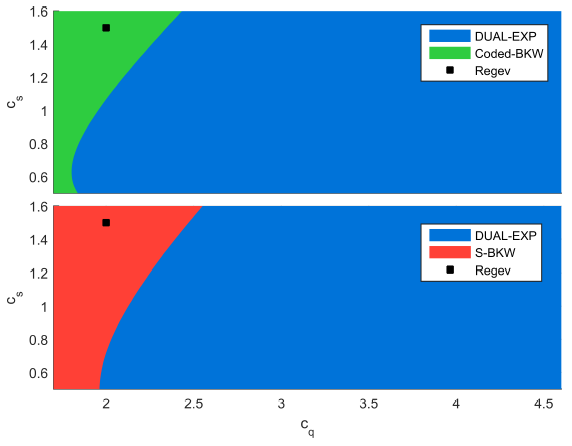
\includegraphics[scale=0.5]{1.png}\\
Рис. 1. Сравнение асимптотического поведения лучших одно-показательных алгоритмов для решения задачи LWE для различных значений $c_q$ и $c_s$. Различные области показывают, где в пространстве параметров соответствующий алгоритм превосходит другие алгоритмы на этом участке.
\end{center}

Пример цитирования статьи \cite{KF15}.


%------- Bibliography -----------

\def\shortbib{1}
\bibliographystyle{alpha}
\bibliography{mybib}

\end{document}